\documentclass{beamer}
\usepackage[brazil]{babel}
\usepackage[T1]{fontenc}
\usepackage[utf8]{inputenc}
\usepackage{url}
\usepackage{bibentry}
\usepackage{graphicx}
\usepackage[alf]{abntex2cite}
\usepackage{booktabs}

% \usetheme{Warsaw}
\usetheme{CambridgeUS}
\usecolortheme{dolphin}
\useoutertheme[footline=authortitle]{miniframes}
 
\begin{document}
 
\title[IFRN - CNAT]
      {Relatório Técnico de Desenvolvimento da Biblioteca Mirobot-Poti}
      \author[Mateus Oliveira Costa Bezerra]
             {Mateus Oliveira Costa Bezerra \\ Orientador: Prof. Me. Leonardo Ataide Minora}
  \institute{Instituto Ferderal de Educação, Ciência e Tecnologia do Rio Grande
    do Norte \\ Campus Natal-Central}
  \date{14 de fevereiro de 2017}

\begin{frame}
  \label{capa}
  \maketitle
\end{frame}

\begin{frame}
  \label{sumario}
  \frametitle{Sumário}
  \tableofcontents
  
\end{frame}

\begin{frame}
  \label{tangivel}
  \section{Introdução}
  \subsection{Programação Tangível}
  \frametitle{Programação Tangível: AlgoBlock}
       \begin{center}
         \begin{figure}
           
         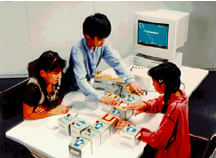
\includegraphics[width=8cm]{imagens/tangible.png}
          \caption{\tiny AlgoBlock(1992) Suzuki e H. Kato}
         \end{figure}


     \end{center}
\end{frame}


 
\begin{frame}
  \frametitle{Programação Tangível: Logo}
  \begin{center}
    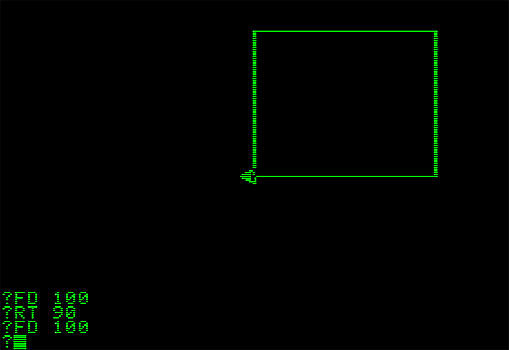
\includegraphics[width=8cm]{imagens/logo1.jpg}
    \end{center}
\end{frame}

\begin{frame}
  \frametitle{Programação Tangível: Logo}
  \begin{center}
    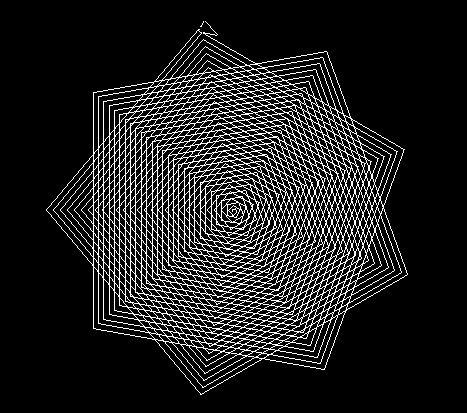
\includegraphics[width=8cm]{imagens/logo2.png}
  \end{center}
\end{frame}


\begin{frame}
  \frametitle{Programação Tangível}
  \begin{block}{Conceito}
    \begin{itemize}
    \item Programação Tangível se a refere a atividade de arranjar os blocos para \textbf{construir}(no sentido oposto de ``escrever'') programas de computador. ~\cite{McNerney2000}
    \end{itemize}
  \end{block}
  
  \begin{block}{Principal Caracteristica}
    \begin{itemize}
    \item Diferente de manipular objetos virtuais, você manipula objetos reais para se comunicar com o computador.
    \end{itemize}
    \end{block}  
\end{frame}

\begin{frame}
  \label{mirobot}
  \subsection{Robô Mirobot}
  \frametitle{Robô Mirobot}
  
  \begin{center}
    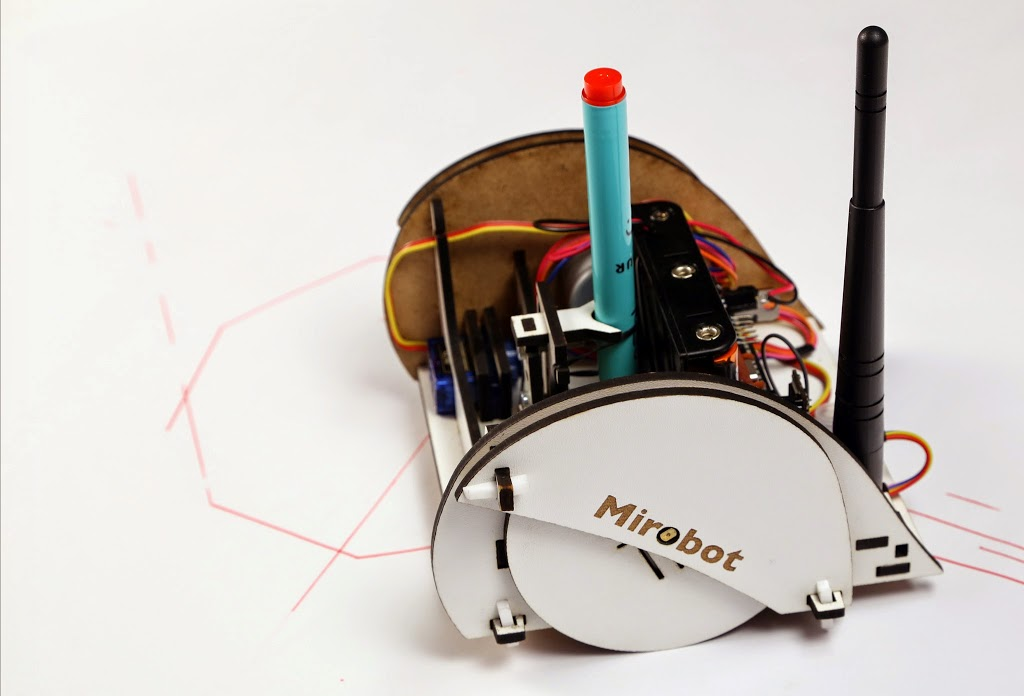
\includegraphics[width=10cm]{imagens/mirobot.jpg}
  \end{center}

\end{frame}

\begin{frame}
  \label{Potigol}
  \subsection{Potigol}
  \frametitle{Potigol}
  \begin{block}{História ~\cite{HellenLemos}}
        \begin{itemize}
    \item Projeto iniciado no ano de 2011 no IFRN - CNAT.
    \item Prof. Leonardo Reis Lucena.
     \item Aplicação nos cursos técnicos e superiores.  
        \end{itemize}

  \end{block}
  
        \begin{block}{Características}
          \begin{itemize}
          \item Sintaxe em \textbf{português}.
          \item Suporte multiparadigma.
          \item Planejada para ser usada por alunos iniciantes.
          \item Funciona dentro da JVM.
          \end{itemize}
        \end{block}
\end{frame}

\begin{frame}
  \section{Objetivo Geral do Trabalho}
  \frametitle{Objetivo Geral do Trabalho}
  \begin{center}
\Large    Implementar uma biblioteca que permita programar na linguagem Potigol comportamentos de um robô Mirobot.
  \end{center}
\end{frame}

\begin{frame}
  \section{Desenvolvimento da Biblioteca}
  \subsection{Protocolo do Robô Mirobot}
  \label{protocolo}
  \frametitle{Protocolo do Robô Mirobot: WebSocket}

  % WebSocket

  \begin{block}{WebSocket ~\cite{websocket2011}}
    \begin{itemize}
    \item Possibilita comunicação bi-direcional.
    \item Funciona sobre o protocolo TCP.
    \item O objetivo principal dessa tecnologia é prover um mecanismo para aplicações que funcionam em  browsers e que precisam de comunicação bi-direcional.
      \item Glassfish Tyrus.
    \end{itemize}
  \end{block}
  
\end{frame}

 \begin{frame}
   \frametitle{Protocolo do Mirobot: Exemplos de Comandos do Mirobot}
     \begin{center}
\bgroup
\def\arraystretch{1.3}
       \begin{tabular}{| c | c | c |}
         \hline
\multicolumn{3}{ |c| }{\large \textbf{Comandos do Mirobot} \small \textcolor{blue}{~\cite{Mime}}} \\ \hline
         \textbf{Comando} & \textbf{Argumento}  & \textbf{Tipo} \\ \hline
         version & nenhum & curto \\
         ping & nenhum & curto \\
         forward & valor em mm & longo \\
         back & valor em mm & longo \\
         left & valor em graus & longo \\
         rigth & valor em graus & longo \\
         pendown & nenhum & longo \\
         penup & nenhum & longo \\
        \hline
       \end{tabular}
    \egroup
 \end{center}

%% %  \end{center}
%%   % Ações do Mirobot
 \end{frame}

\begin{frame}
   \frametitle{Protocolo do Mirobot: Formatação das Mensagens}

   \begin{block} {JSON Recebido pelo Mirobot}
     \begin{itemize}
     \item \textbf{cmd}: O comando que irá ser executado.
     \item \textbf{arg}: Algum argumento para o comando(se necessário).
     \item \textbf{id}: Uma string para identificar o comando na hora de receber a resposta.
     \end{itemize}
   \end{block}

   \begin{block} {JSON Enviado pelo Mirobot}
     \begin{itemize}
     \item \textbf{status}: A situação do comando que foi recebido.
     \item \textbf{msg}: Algum dado que foi requisitado.
     \item \textbf{id}: O identificador da mensagem a qual esta sendo respondida.
     \end{itemize}
   \end{block}
\end{frame}

\begin{frame}
   \frametitle{Protocolo do Mirobot: Formatação das Mensagens}

   \begin{center}
     Comando JSON recebido pelo mirobot:
     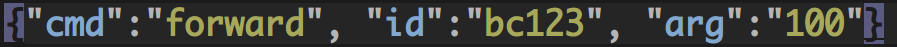
\includegraphics[width=12cm]{imagens/json1.png} \\

     Comando JSON enviado pelo Mirobot:
     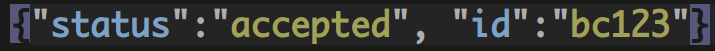
\includegraphics[width=10cm]{imagens/json2.png}
   \end{center}

\end{frame}

\begin{frame}
  \subsection{Implementação dos Métodos da Classe Mirobot}
  \label{implementacao}
  \frametitle{Implementação dos Métodos da Classe Mirobot}

  \begin{block}{Etapas da Implementação}
    \begin{itemize}
    \item Definição dos nomes dos métodos da classe Mirobot.
    \item Importação de um arquivo .JAR no Potigol e testes.
    \item Criação da classe intermediária entre a classe Mirobot e o robô.
    \item Implementação dos métodos nomeados anteriormente.
    \item Teste do exemplo com simulador do Mirobot.
    \end{itemize}
  \end{block}
\end{frame}

\begin{frame}
  \subsection{Exemplo de Uso da Biblioteca Mirobot-Poti}
  \label{exemplo}
  \frametitle{Exemplo de Uso da Biblioteca Mirobot-Poti}
   \begin{center}
     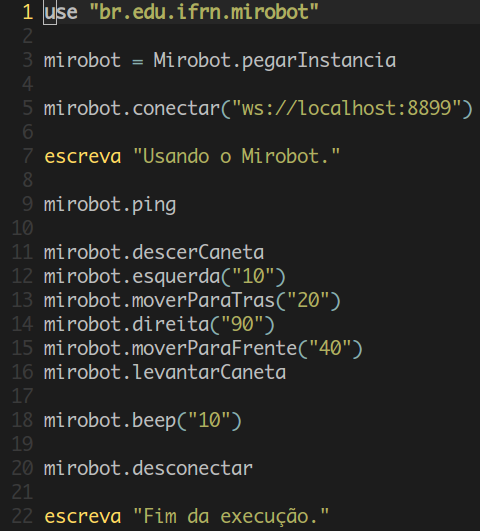
\includegraphics[width=6cm]{imagens/teste-potigol.png}
   \end{center}
\end{frame}

\begin{frame}
  \label{consideracoes}
  \section{Considerações Finais}
  \frametitle{Considerações Finais}
    \begin{itemize}
    \item Príncipais Contribuições.
    \item Limitações e Dificuldades.
    \item Trabalhos Futuros.
    \end{itemize}
\end{frame}

\begin{frame}
  \label{referencias}
  \section{Referências}
  \frametitle{Referências}
  \bibliographystyle{abntex2-alf}
  \bibliography{Referencias}
\end{frame}

\end{document}
